\chapter{Deepfake methods}
\section{Autoencoder}
Autoencoders are the most basic approach to the problem of deepfake generation. In fact, all mentioned methods are just different variations of this idea. Autoencoder is a type of artificial neural network that learns to reproduce given input in an unsupervised manner. The problem is to train functions \(A: \mathbb{R}^n \to \mathbb{R}^p\) (encoder) and \(B: \mathbb{R}^p \to \mathbb{R}^n\) (decoder) to satisfy condition given in equation \ref{eq:autoencoder_condition} as described in \cite{autoencoders_bib},
%
\begin{equation}
\label{eq:autoencoder_condition}
arg \, min_{A,B} E[\Delta(x,B \circ A(x))]
\end{equation}
%
where \(E\)-- expectation over the distribution of \(x\) and \(\Delta\)-- reconstruction loss function, which measures the distance between given input and the output of the decoder. General idea of autoencoder model is illustrated in figure \ref{fig:autoencoder_general_idea}. Typically, architecture of autoencoder consists not only of input and output layers, as this would result in simple coping pixels from the input to the output of the network, but also contains single or multiple hidden layers in between, with the number of neurons lesser than the number of pixels in the input image. Such structure causes bottleneck effect and creates so-called compressed representation at the output of the encoder part, known also as ``feature map'' or in case of deepfake ``latent face''. Such compression causes feature map to preserve only information most relevant for later reconstruction and gets rid of unnecessary data.

\begin{figure}[H]
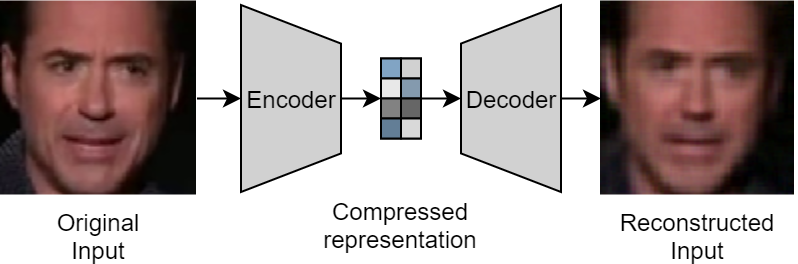
\includegraphics[width=12cm] {autoencoder_general_idea.png}
\centering
\caption{Autoencoder general idea}
\label{fig:autoencoder_general_idea}
\end{figure}

Generating deepfakes using autoencoders approach consists of three major steps. Described process is illustrated in figure \ref{fig:deepfake_steps}. Let us assume that \(X\) is a set of face images of person \(x\) and \(Y\) is a set of face images of person \(y\). Firstly, as shown in figure \ref{subfig:deepfake_steps_a}, an encoder is trained to produce feature maps for images of face from both classes. Afterwards, two decoders are trained separately to reproduce original images from latent faces generated by pre-trained encoder, as presented in figure \ref{subfig:deepfake_steps_b}. Finally, decoders are switched to produce images from one class based on feature maps from the other class, which was illustrated in figure \ref{subfig:deepfake_steps_c}.

\begin{figure}[H]
\centering
\begin{subfigure}{12cm}
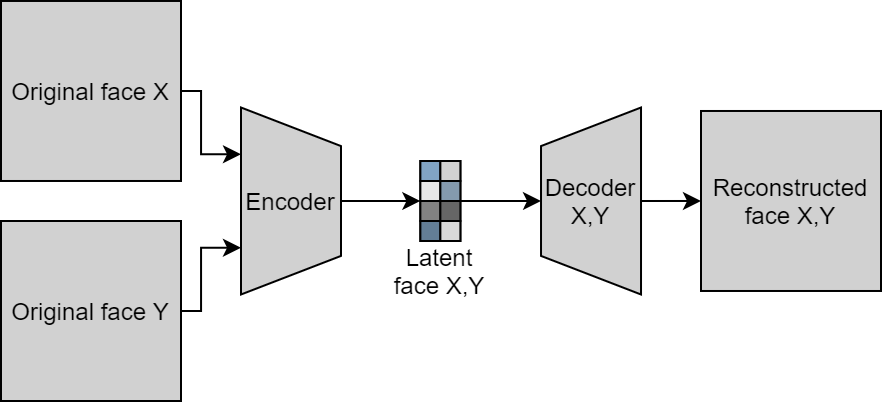
\includegraphics[width=\textwidth]{deepfake_idea_1.png}
\caption{Training autoencoder}
\label{subfig:deepfake_steps_a}
\end{subfigure}

\begin{subfigure}{12cm}
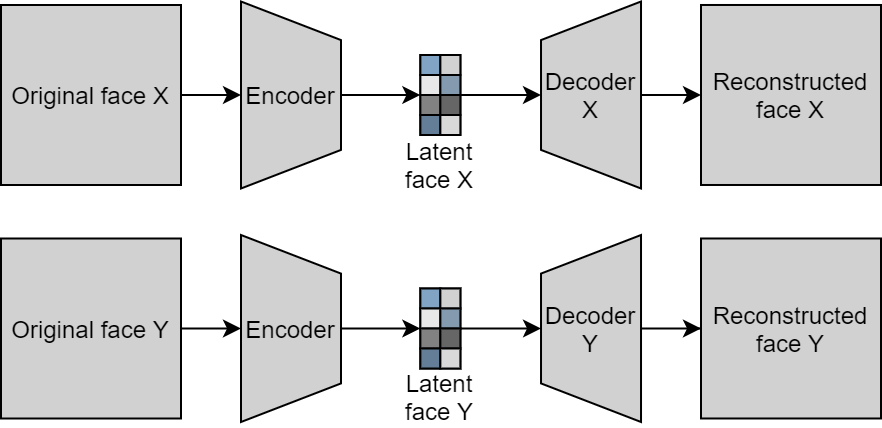
\includegraphics[width=\textwidth]{deepfake_idea_2.png}
\caption{Training decoders X and Y}
\label{subfig:deepfake_steps_b}
\end{subfigure}

\begin{subfigure}{12cm}
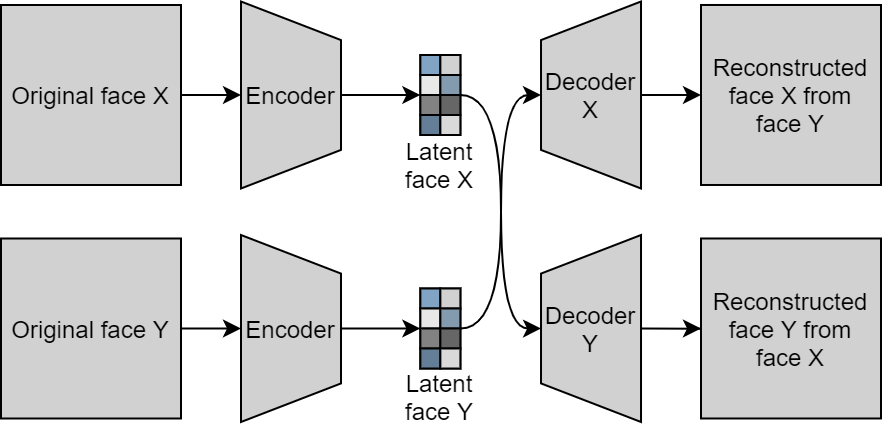
\includegraphics[width=\textwidth]{deepfake_idea_3.png}
\caption{Generating X from Y and Y from X}
\label{subfig:deepfake_steps_c}
\end{subfigure}

\caption{Three steps of generating deepfakes}
\label{fig:deepfake_steps}
\end{figure}

\section{Variational autoencoder}
Idea behind deepfake generated by VAE with CNN

\section{VAE-GAN}
Idea behind deepfake generated by GAN actually ''VAE-GAN''.

\section{CycleGAN}
Describe what is it, what it consists of, what are its applications, why I thought it should work for deepfake. Explain how it works exactly. Show learning process and results (good ones: horses to zebras and bad ones: face to face). Idea behind deepfake generated by CycleGAN. Explain why I'm assuming it should it work?